\chapter{Практические задания}

\section{Задание 1}
В таблице 0.1 приведены выражения и результат их вычисления.
\begin{table}[H]
    \centering
    \caption{Результаты вычисления выражений задания \No{}1}
	\begin{tabular}{|c|c|}
 	\hline
    Выражение & Результат \\
 	\hline
 	(caadr '((blue cube) (red pyramid))) & red \\
 	\hline
 	(cdar '((abc) (def) (ghi))) & nil \\
 	\hline
    (cadr '((abc) (def) (ghi))) & (def) \\
 	\hline
    (caddr '((abc) (def) (ghi))) & (ghi) \\
 	\hline
	\end{tabular}
\end{table}

\section{Задание 2}
\begin{table}[H]
    \centering
    \caption{Результаты вычисления выражений задания \No{}2}
	\begin{tabular}{|c|c|}
 	\hline
    Выражение & Результат \\
 	\hline
 	(list 'Fred 'and Wilma) & ошибка \\
 	\hline
    (list 'Fred '(and Wilma)) & (FRED (AND WILMA))\\
 	\hline
    (cons nil nil) & (NIL) \\
 	\hline
    (cons t nil) & (T) \\
 	\hline
    (cons nil t) & (NIL .T)\\
 	\hline
    (list nil) & (NIL) \\
 	\hline
    (cons (t) nil) & ошибка \\
 	\hline
    (list '(one two) '(free temp)) & ((ONE TWO) (FREE TEMP)) \\
 	\hline
    (cons 'Fred '(and Wilma)) & (FRED AND WILMA) \\
 	\hline
    (cons 'Fred '(Wilma)) & (FRED WILMA) \\
 	\hline
    (list nil nil) & (NIL NIL) \\
 	\hline
    (list t nil) & (T NIL) \\
 	\hline
    (list nil t) & (NIL T) \\
 	\hline
    (cons t (list nil)) & (T NIL) \\
 	\hline
    (list (t) nil) & ошибка \\
 	\hline
    (cons '(one two) '(free temp)) & ((ONE TWO) FREE TEMP) \\
 	\hline
	\end{tabular}
\end{table}
В таблице 0.2 приведены выражения и результат их вычисления.

\section{Задание 3}
В листинге 1 приведён текст трёх функций, а в комментариях под каждой функцией - значение, которое она возвращает.

\lstset{language=lisp}
\begin{lstlisting}[caption={Примеры функций, возвращающих списки}]
(defun f1 (ar1 ar2 ar3 ar4)
  (list (list ar1 ar2) (list ar3 ar4)))
; ((ar1 ar2) (ar3 ar4))

(defun f2 (ar1 ar2)
  (list (list ar1) (list ar2)))
; ((ar1) (ar2))

(defun f3 (ar1)
  (list (list (list ar1))))
; (((ar1)))
\end{lstlisting}

На рисунках 0.1-0.3 изображены списочные ячейки результатов рассмотренных выше функций.

\begin{figure}[H]
    \centering
    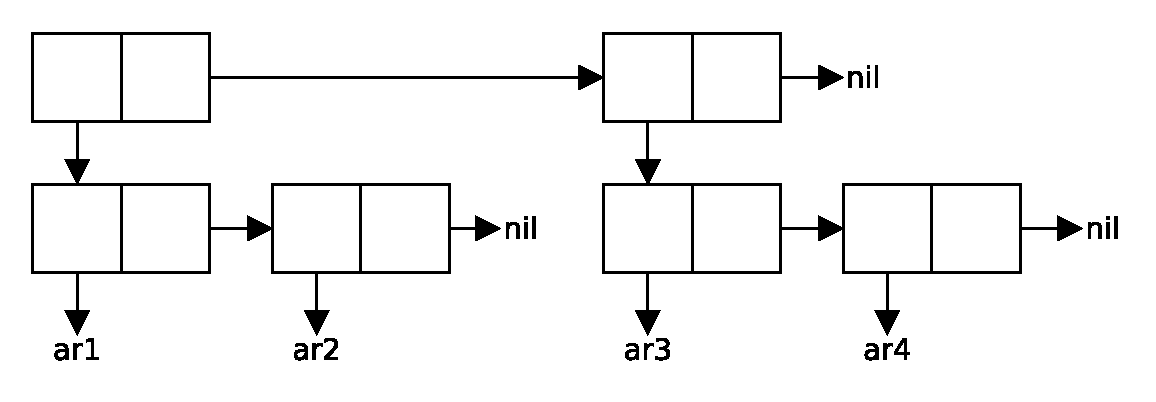
\includegraphics[scale=0.75]{data/pdf/02-01.pdf}
    \caption{Список ((ar1 ar2) (ar3 ar4))}
\end{figure}

\begin{figure}[H]
    \centering
    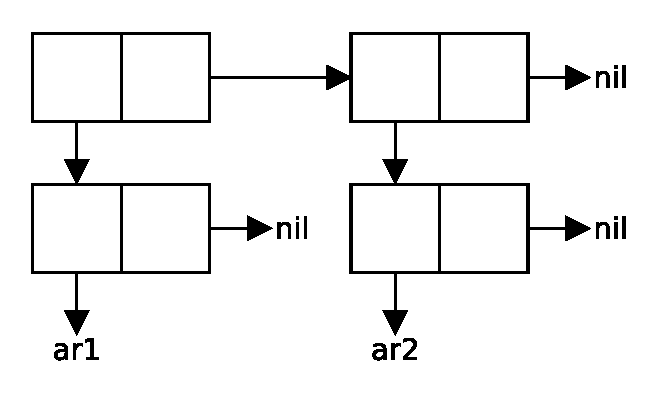
\includegraphics[scale=0.75]{data/pdf/02-02.pdf}
    \caption{Список ((ar1) (ar2))}
\end{figure}

\begin{figure}[H]
    \centering
    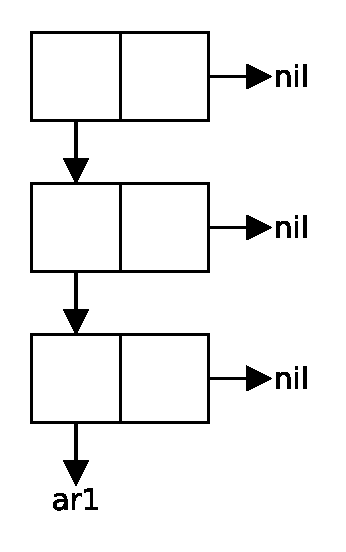
\includegraphics[scale=0.75]{data/pdf/02-03.pdf}
    \caption{Список (((ar1)))}
\end{figure}

